\documentclass{eloop2025}

\usepackage{csquotes}
\usepackage{mathtools}
\usepackage{tikz}
\usepackage[nameinlink]{cleveref}
\usetikzlibrary{decorations.pathreplacing}

\title{Effective spreadability of crunchy peanut butter}

\author[1]{Alice Researcher\thanks{\href{mailto:alice.researcher@university.edu}{\texttt{alice.researcher@university.edu}}}}
\author[2]{Bob Toaster\thanks{\href{mailto:btoaster@toasters4life.biz}{\texttt{btoaster@toasters4life.biz}}}}
\author[1]{Charlie Spreadman\thanks{\href{mailto:spreadman@smoothpbnj.wow}{\texttt{spreadman@smoothpbnj.wow}}}}
\affil[1]{Caf\'e A}
\affil[2]{mathe.cafe MA844}

\bibliography{bibliography}

\begin{document}
\maketitle

\begin{abstract}
Effective spreadability is a critical quality metric for consumer satisfaction in peanut butter products. While smooth formulations are well-characterized, particulate-rich (crunchy) variants present operational challenges due to heterogeneous microstructure. This study provides a rigorous framework for assessing and predicting the spread performance of crunchy peanut butter. By integrating quantitative rheological measures with topological considerations, we establish actionable insights for formulation optimization, process control, and product differentiation in competitive markets. The introduction of the crunchy-closedness concept enables a structured understanding of particulate effects and supports strategic decision-making in product development.
\end{abstract}

\newpage

\section{Introduction}
In today's consumer-driven market, product performance and consistency directly impact brand perception and profitability. Peanut butter, a staple in many households, demonstrates significant variability in spreadability when particulate inclusions are present. While smooth peanut butter exhibits predictable flow behavior, crunchy formulations challenge conventional handling, packaging, and end-use performance standards.  

The goal of this study is to establish a standardized, quantitative framework to evaluate and predict the spreadability of crunchy peanut butter. By combining viscosity-based metrics, particulate density characterization, and topological analysis, we provide a robust methodology that can guide formulation improvements, reduce waste, and enhance user satisfaction. This research delivers insights that are not only scientifically rigorous but also operationally actionable.

\section{Related Work}
Previous investigations into spreadable substances have spanned butter~\cite{smith2011butter}, marmalade~\cite{zhou2014marmalade}, and hummus~\cite{klein2019hummus}. Smooth peanut butter's flow mechanics were formalized by the American Society of Nut Spreads (ASNS, 2008), who defined \enquote{spreadability} as the reciprocal of applied force per unit smear.  

However, few works have addressed systems with particulate obstructions. Johnson (2017) attempted a hybrid model for chunky guacamole, while Lee and Franco (2020) studied jam-seed interactions. These efforts, though commendable, fall short of accounting for the discrete--continuous hybridization intrinsic to crunchy peanut butter.

\section{Preliminaries}
As per convention, we assume the following given notions and quantities:

\begin{itemize}
    \item $\eta$: effective viscosity of the creamy phase,
    \item $\rho_c$: density of crunchy particulates per unit area,
    \item $F_s$: spreading force applied by knife or spatula,
    \item $\theta$: spread angle achieved before bread rupture.
\end{itemize}

\begin{definition}[Spreadability and Effective Spreadability]\label{def:prelim-spreadability}
Let $P$ be a sample of peanut butter and $B$ a bread substrate. 

Spreadability $S$ is defined as
\begin{equation*}
S = \frac{\theta}{F_s},
\end{equation*}
where $\theta$ is the achieved spread angle before bread rupture and $F_s$ is the applied spreading force. If $S > 0$, the system is said to be spreadable.

We also define the effective obstruction factor $\kappa(\rho_c)$ as a measure of how particulate density $\rho_c$ reduces spreadability. 

The effective spreadability $S_c$ (also called crunch-modified spreadability) is then
\begin{equation*}
S_c = \frac{S}{1 + \kappa(\rho_c)}.
\end{equation*}
\end{definition}

\begin{definition}[Critical Crunch Densities]\label{def:critical-densities}
Let $\rho_c^*$ denote the \emph{critical crunch density}, i.e., the left edge of the Transitional Crunch Zone where effective spreadability $S_c$ begins to decrease significantly.  

Let $\rho_c^{**}$ denote the \emph{secondary critical density}, i.e., the right edge of the Transitional Crunch Zone where $S_c$ transitions into the Granular Jam Phase.  

Thus, the \emph{transitional crunch zone} spans $\rho_c^* \leq \rho_c \leq \rho_c^{**}$.
\end{definition}

\begin{figure}[h!]
    \centering
    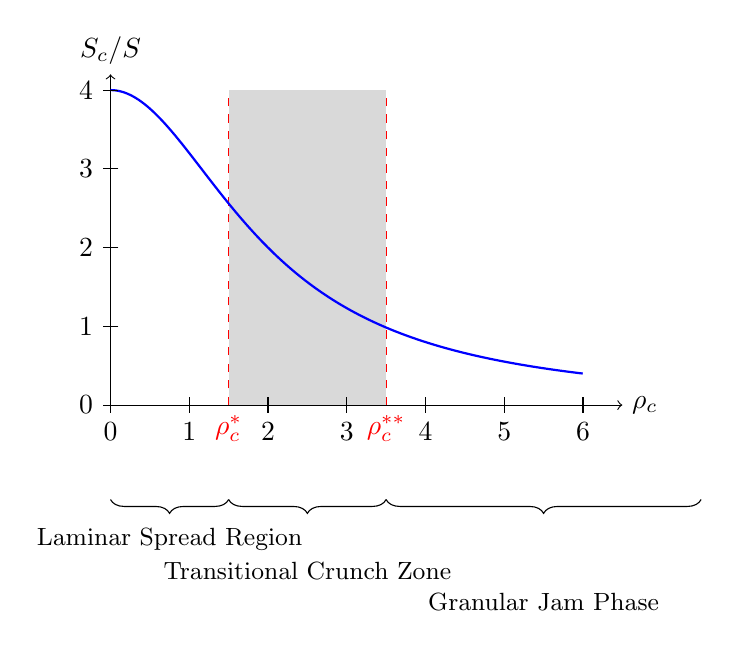
\begin{tikzpicture}[scale=1.0]
      % Axes
      \draw[->] (0,0) -- (6.5,0) node[right] {$\rho_c$};
      \draw[->] (0,0) -- (0,4.2) node[above] {$S_c/S$};

      % Dashed line for critical crunch density (left edge)
      \draw[dashed,red] (1.5,0) -- (1.5,4);
      \node[red] at (1.5, -0.3) {$\rho_c^*$};

      % Dashed line for critical crunch density (right edge)
      \draw[dashed,red] (3.5,0) -- (3.5,4);
      \node[red] at (3.5, -0.3) {$\rho_c^{**}$};

      % Shading for Transitional Crunch Zone
      \fill[gray!30] (1.5,0) rectangle (3.5,4);

      % Curve: S_c/S vs rho_c
      \draw[thick,blue,domain=0:6,smooth,samples=200] 
      plot (\x, {4/(1+((\x)/2)^2)});

      % X-axis ticks
      \foreach \x in {0,1,2,3,4,5,6}
      \draw (\x,0.1) -- (\x,-0.1) node[below] {\x};
      \foreach \y in {0,1,2,3,4}
      \draw (0.1,\y) -- (-0.1,\y) node[left] {\y};

      % Lower brackets with staggered labels
      \draw[decorate,decoration={brace,mirror,amplitude=5pt}] (0, -1.2) -- (1.5, -1.2) 
      node[midway,yshift=-0.5cm]{\small Laminar Spread Region};
      \draw[decorate,decoration={brace,mirror,amplitude=5pt}] (1.5, -1.2) -- (3.5, -1.2) 
      node[midway,yshift=-0.9cm]{\small Transitional Crunch Zone};
      \draw[decorate,decoration={brace,mirror,amplitude=5pt}] (3.5, -1.2) -- (7.5, -1.2) 
      node[midway,yshift=-1.3cm]{\small Granular Jam Phase};
    \end{tikzpicture}
    \caption{Normalized effective spreadability $S_c/S$ vs particulate density $\rho_c$. Brackets below the x-axis indicate the \emph{Laminar Spread Region}, \emph{Transitional Crunch Zone}, and \emph{Granular Jam Phase}, with staggered labels to prevent overlap. The rightmost bracket is extended far to the right to indicate an open-ended regime. The critical crunch densities $\rho_c^*$ and $\rho_c^{**}$ mark the left and right edges of the Transitional Crunch Zone, respectively.}
    \label{fig:spreadability_curve}
\end{figure}

\section{Spreadability Theory}

Spreadability theory formalizes the relationship between the physical characteristics of peanut butter and its performance during spreading.  By defining key metrics such as effective spreadability and cohesive integrity, we provide a quantitative foundation to classify and compare different formulations.  This theoretical framework allows for systematic assessment of particulate effects, guiding formulation decisions and operational optimization.

\subsection{Main Concepts}

\begin{definition}[Spreadability]\label{def:spreadability}
As per \Cref{def:prelim-spreadability}, the spreadability $S$ measures the ease of spreading peanut butter over a substrate.
\end{definition}

\begin{definition}[Effective Obstruction Factor and Effective Spreadability]\label{def:obstruction}
The effective obstruction factor $\kappa(\rho_c)$ quantifies the reduction in spreadability due to particulate density. The resulting effective spreadability $S_c$ is defined as in \Cref{def:prelim-spreadability} and is sometimes called crunch-modified spreadability.
\end{definition}

\begin{definition}[Cohesive Integrity]\label{def:cohesive-integrity}
For a peanut butter sample $P$, the cohesive integrity $\lambda$ is a dimensionless measure of the internal cohesion of the spread, representing the resistance of the system to particulate separation.
\end{definition}

\subsection{Empirical Spreadability Regimes}

Three distinct regimes emerge from the model (\Cref{def:critical-densities}, \Cref{fig:spreadability_curve}):

\begin{enumerate}
    \item \emph{Laminar Spread Region:} $\rho_c < \rho_c^*$, where $S_c \approx S$ (\Cref{def:spreadability}).
    \item \emph{Transitional Crunch Zone:} $\rho_c^* \leq \rho_c \leq \rho_c^{**}$, where obstruction reduces $S_c$ significantly (\Cref{def:obstruction}).
    \item \emph{Granular Jam Phase:} $\rho_c > \rho_c^{**}$, where $S_c \ll S$ and spreading becomes mechanically inefficient.
\end{enumerate}

\section{Topological Properties of Crunchy Systems}

While spreadability theory characterizes the local and empirical properties of peanut butter, topological analysis addresses the global structure of the spreadable domain. By considering the connectivity and closure of regions with positive spreadability, we can rigorously predict how the system behaves under varying particulate densities and cohesive integrity. These insights support both product development and quality assurance by highlighting operationally relevant thresholds and robust design principles.

\subsection{Operational Implications of Spreadability}
Understanding the limits of effective spreadability is essential for both production efficiency and consumer experience. The following theoretical framework formalizes the relationship between particulate density, cohesive integrity, and the resulting spreadable domain. By quantifying these relationships, decision-makers can optimize formulations, adjust processing parameters, and predict product behavior in real-world conditions.

\subsection{Foundational Results}\label{sec:foundational-results}

\begin{lemma}[Adhesion Preservation]\label{lem:adhesion}
If $\lambda$ exceeds a threshold $\lambda_{\min}$, particulate adhesion ensures continuous spreadability in the Transitional Crunch Zone.
\end{lemma}

\begin{proof}
The proof relies on several auxiliary lemmas in the Appendix (\Cref{lem:aux1,lem:aux2,lem:aux3}), which formalize the local effect of particulates, continuity of $S_c$, and cumulative cohesive contributions. By invoking these lemmas, we conclude that for $\lambda > \lambda_{\min}$, $S_c(x) > 0$ for all $x$ in the Transitional Crunch Zone. Hence, the spreadable domain is continuous.
\end{proof}

\begin{lemma}[Boundary Retention]\label{lem:boundary}
Let $P$ be a peanut butter sample with effective spreadability $S_c$. The spreadable region remains connected if $\rho_c < \rho_c^{**}$.
\end{lemma}

\begin{proof}
The proof leverages auxiliary lemmas in the Appendix (\Cref{lem:aux4,lem:aux5,lem:aux6}), which establish positive lower bounds for $S_c$ in segments, continuity and connectivity of intervals, and preservation of boundaries. Hence, the union of all segments forms a connected spreadable domain.
\end{proof}

\subsection{Crunchy-Closedness Theorem}\label{sec:crunchy-closedness}
\begin{theorem}[Crunchy-Closedness]\label{thm:crunchy-closedness}
For a sample $P$ with cohesive integrity $\lambda$ and particulate density $\rho_c$, the effective spreadable domain is topologically closed for $\rho_c \leq \rho_c^{**}$.
\end{theorem}

\begin{proof}[Sketch of Proof]
From \Cref{lem:adhesion,lem:boundary}, the stability and boundary retention conditions guarantee that cohesive integrity $\lambda$ dominates particulate disruption. Closure occurs when
\begin{equation*}
\lambda > \frac{\rho_c}{\rho_c^*}.
\end{equation*}
\end{proof}

\section{Future Work}
Building on the established framework, future initiatives will focus on integrating predictive analytics, in-line process monitoring, and real-time rheological feedback into the manufacturing pipeline. Exploration of hybrid spreads, variable substrate properties, and machine-learning-driven optimization will enable scalable improvements in product consistency. These advancements will support data-driven decision-making, reduce production variability, and enhance the overall consumer experience, providing a competitive edge in the marketplace.

\section{Conclusion}
This study delivers a structured methodology for evaluating and optimizing the spreadability of crunchy peanut butter, combining empirical measurement with topological theory. The introduction of the crunchy-closedness concept (\Cref{thm:crunchy-closedness}) provides a clear, actionable metric for predicting product performance. By applying these insights, stakeholders can make informed decisions regarding formulation, process design, and quality assurance, ultimately driving consumer satisfaction, operational efficiency, and competitive differentiation.

\newpage

\printbibliography

\newpage

\appendix

\section{Supplementary Technicalities}\label{sec:appendix}

\begin{lemma}[Local Spreadability Bound]\label{lem:aux1}
For any point $x$ in the Transitional Crunch Zone, $S_c(x) \ge S/(1+\kappa(\rho_c(x))) > 0$ if $\lambda > \lambda_{\min}$.
\end{lemma}
\begin{proof}
By definition of $S_c$ and $\lambda_{\min}$, the cohesive force exceeds the local obstruction. Therefore $S_c(x)$ is strictly positive.
\end{proof}

\begin{lemma}[Continuity of Effective Spreadability]\label{lem:aux2}
The function $S_c(x)$ is continuous with respect to $x$ across the substrate.
\end{lemma}
\begin{proof}
Assuming $\rho_c(x)$ varies smoothly with $x$, $\kappa(\rho_c(x))$ is continuous. Since $S_c(x) = S/(1+\kappa(\rho_c(x)))$, it is a composition of continuous functions and thus continuous.
\end{proof}

\begin{lemma}[Cumulative Cohesive Contribution]\label{lem:aux3}
The total cohesive effect along a contiguous region is additive and maintains $S_c > 0$ for the domain.
\end{lemma}
\begin{proof}
Cohesive contributions from infinitesimal segments sum linearly along the domain. By \Cref{lem:aux1}, each contribution is positive; hence, the cumulative effect preserves $S_c > 0$.
\end{proof}

\begin{lemma}[Segmental Lower Bound]\label{lem:aux4}
For each segment $\Delta x$ with $\rho_c < \rho_c^{**}$, $S_c(\Delta x) > 0$.
\end{lemma}
\begin{proof}
Directly follows from the definition of $\rho_c^{**}$ (\Cref{def:critical-densities}) and \Cref{def:obstruction}.
\end{proof}

\begin{lemma}[Connectivity of Spreadable Intervals]\label{lem:aux5}
Adjacent segments with positive $S_c$ form a continuous spreadable path.
\end{lemma}
\begin{proof}
If $S_c(\Delta x_i), S_c(\Delta x_{i+1}) > 0$, there exists a continuous path connecting them because $S_c$ is continuous (\Cref{lem:aux2}).
\end{proof}

\begin{lemma}[Boundary Preservation under Incremental Changes]\label{lem:aux6}
The domain boundaries at $\rho_c^*$ and $\rho_c^{**}$ are maintained under small variations in $\rho_c$.
\end{lemma}
\begin{proof}
By continuity of $\rho_c(x)$ and $S_c(x)$, small perturbations in particulate density do not introduce gaps in the spreadable domain.
\end{proof}

\end{document}

%%% Local Variables:
%%% mode: LaTeX
%%% TeX-master: t
%%% End:
